

    而后将始终只考虑这种定向的正交归一基。

一个具有确定指向的、时间定向的正交基就是\textit{惯性基矢},由于矢量空间和闵氏背景本身的等同,我们就可以把这些矢量都“搬”到闵氏时空里来。

一般认为所考虑的惯性系(进而惯性基矢)都应具备一致时间定向。
    


惯性坐标系一般就选择处处与参考系标架一致的坐标基,可统称惯性系。

因为参考系由充斥于时空(或其开子集)的无数观者组成,过每一时空点有且仅有一条观者世界线,所以,给定一个参考系后,全时空(或其开子集)就有一个 4-标架场。任何时空点的任何张量都可用该点的4-标架作为基底表出。
\begin{definition}[观者]
    观者指一条定义了4-标架场 $\{e_\mu\}$ 的类时世界线,并规定
    \eq{
    g(e_\mu,e_\nu)=\eta_{\mu\nu},\quad e_0=Z.
    }
    这里 $g$ 是时空所配度规,闵氏时空取 $\upeta$。
\end{definition}
世界线为测地线的运动就称为\textit{惯性运动},则对惯性观者的准确定义是:
\begin{definition}[惯性观者]
    惯性观者是做惯性运动的无自转观者。
\end{definition}

决定一个瞬时观者的要素除 $p,Z$外,有时还要辅以 3-标架,它们与 $Z$ 组成$p$点的正交4-标架$\{e_\mu\}$,在此情况下一个瞬时观者应表为
\[(p,\{e_\mu\}),\]
其中 $e_0=Z$。不必强调标架时,瞬时观者仍可表为$(p,Z)$。


关键在于何种情况不仅使得保内积,还使得轴“不动”。不妨这样设想,非测地线意味着 3-速在变化,进而一点的瞬时观者可 boost 到邻近点的另一瞬时观者去,这样,此点观者所持的空间矢量便自然能延至下一观者中去。boost 变换下,$e_\mu$ 间当然能保持正交,说明各点瞬时观者或 4-标架场各点取值间差的正是\textit{无穷小(infinitesimal) boost 变换}。将非测地线看作是一系列瞬时惯性观者的无穷小 boost 变换,轻松使得 $e_i$ 保持其空间性。并且,由于点之间接近,boost 也不包含空间转动(只受 3-速影响),故各 $e_i$ 朝向不变。

$Z,A$ 正交使得 $Z$ 保模长地发生“转动”,因而空间矢量为与之正交而一齐转动。这种转动只涉及到 $Z,A$ 所在(无穷小)平面,此即,boost 变换应是关于 $Z,A$ 平面的伪转动。3 维空间中旋转变换是相关于一个角速度矢量而言的,即
\eq{
\dv{v_i}{\tau}=(\vec\omega\times\vec v)^i=\varepsilon_{ijk}\omega^j v^k,
}
其同时可看作处于 $\vec\omega$ 所对平面上的旋转(按右手螺旋),这个视角在代数上就是在 3 维空间中取其对偶的 2-形式(当然,先用旋转平面的诱导度规降下来),即 $\Omega=\star\vec\omega$,分量为 $\Omega_{ik}=\omega^j\varepsilon_{jik}=-\omega^j\varepsilon_{ijk}$。这样
\eq{
\dv{v^i}{\tau}=(\vec\omega\times\vec v)^i=-\Omega^{ij} v_j,
}
这里旋转平面的特点是同 $\vec\omega$ 垂直,这意味着 $\vec\omega$ 正比于平面上任二线性无关矢量之叉乘,则 $\Omega$ 正比于其楔积。将其推广至高维时,旋转平面有其确切含义(找到两个线性无关矢量),而角速度矢量的对偶不再是平面,故表述上采取 2-形式而非矢量叉乘:
\eq{
\dv{v^\mu}{\tau}=-\Omega^{\mu\nu} v_\nu,
}
此处应将 $\dv*{\tau}$ 理解为惯性坐标系的$D/\d\tau$,而 $\Omega$ 正比于 $A\wedge Z$。令 $v=Z$,则
\[
-\Omega^{\mu\nu} Z_\nu\propto -(A^\mu Z^\nu-Z^\mu A^\nu)Z_\nu=A^\mu=-\Omega^{\mu\nu} Z_\nu.
\]
说明比例系数归一。上式移项后所定义的导数,便满足我们对费移 $D_F v/\d\tau=0$ 的要求。

综上,无自转观者所要求的无非是 4-标架沿线费移。以后谈及等效原理会详述无自转的重要性,如可以避开科氏惯性力之干扰。

\begin{wrapfigure}{l}{.35\textwidth}
    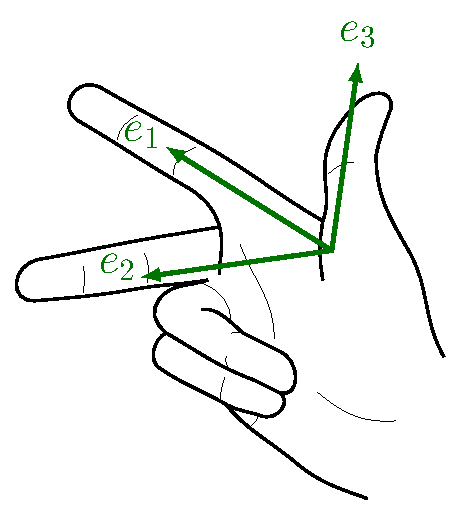
\includegraphics[width=.3\textwidth]{fig/chpt01/tetrad hand.pdf}
    \caption{空间右手 3-标架}
\end{wrapfigure}
还需处处配以\textit{4-标架(tetrad)},也即其上任意点矢量的正交归一基 $\{\bm{e}_\mu\}$,满足 $\bm{e}_\mu\cdot\bm{e}_\nu=\eta_{\mu\nu}$。直观上,\textit{3-标架(frame)}可以是由三根单位长的短直杆或刻度尺焊成的正交架子,每根直杆代表一个观测方向,其在每一时刻的指向由该观者选定。读者亦可尝试用右手大拇指、食指及中指按右手螺旋比划出 3-标架。数学上,3-标架就是空间正交归一基 $\{\bm{e}_i\}$,“空间”指皆与观者世界线切矢 $\bm{e}_0$ 正交。今后谈及 4-标架时默认为右手标架。



因而 4-标架场又称作观者所处处配备的“局部实验室”,所测物理量无非就是将相关的 4 维量投影到 3-标架上。


惯性观者的 4-标架又称\textit{惯性基矢}或\textit{惯性标架}。我们还应希望惯性标架\textit{无自转},否则可能观测到赝力。如图 \ref{k&c},设 Cynthia、Kaylor 两人坐在地面的两把椅子上:Cynthia 坐底座固定的蛋壳椅;Kaylor 坐底座静置的办公椅且不停自转。二者世界线都走直线,但 Cynthia 可视为惯性观者而 Kaylor 不能。
\begin{figure}%
    \centering
    \subfloat[\centering Cynthia]{{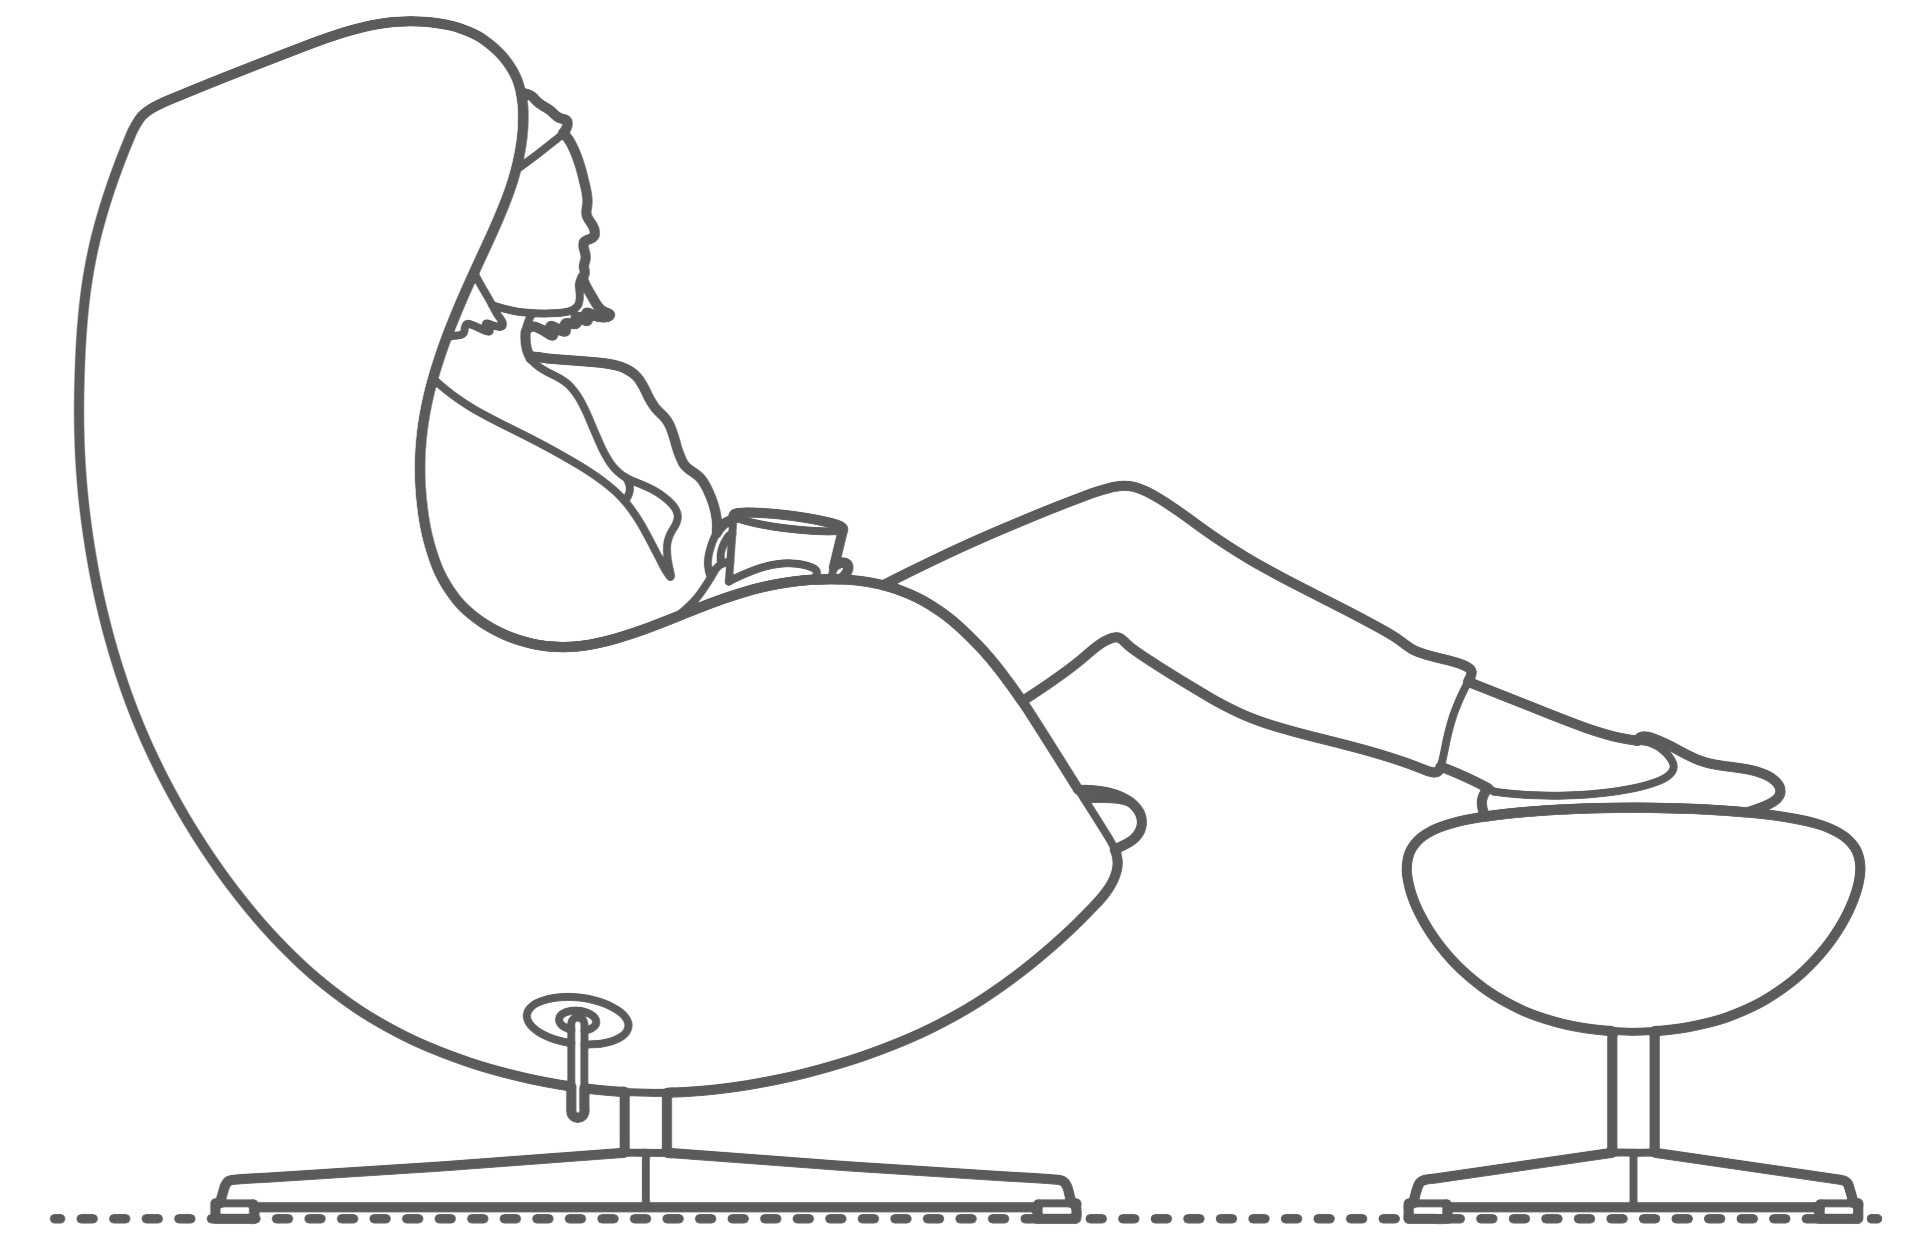
\includegraphics[width=.5\textwidth]{fig/chpt01/eggchair.jpg} }}%
    \subfloat[\centering Kaylor]{{
\tikzset{every picture/.style={line width=0.75pt}} %set default line width to 0.75pt        
\begin{tikzpicture}[x=0.75pt,y=0.75pt,yscale=-.73,xscale=.73]
%uncomment if require: \path (0,300); %set diagram left start at 0, and has height of 300
%Image [id:dp40969400488164953] 
\draw (147,147) node  {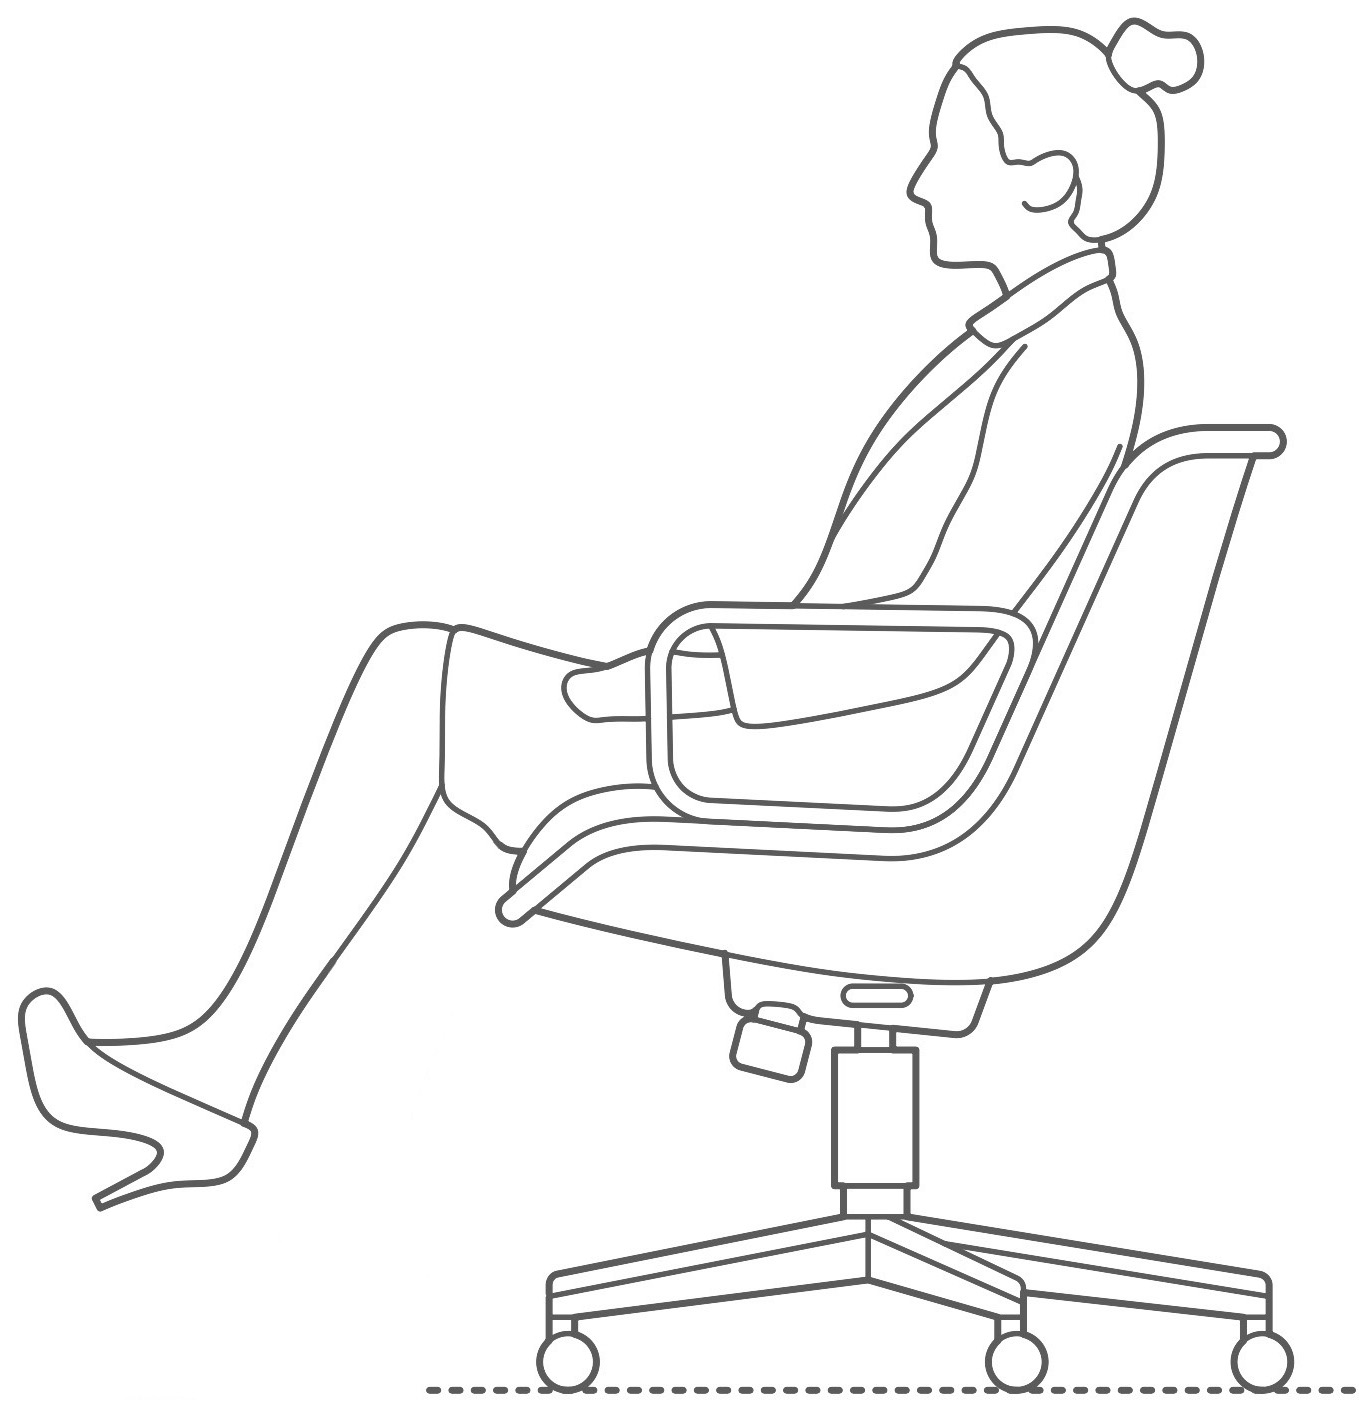
\includegraphics[width=.38\textwidth]{fig/chpt01/rolling.jpg}};
%Shape: Arc [id:dp1232081022977285] 
\draw  [draw opacity=0] (185.25,85.75) .. controls (185.23,85.75) and (185.22,85.75) .. (185.21,85.75) .. controls (142.38,85.75) and (107.67,76.44) .. (107.67,64.96) .. controls (107.67,53.48) and (142.38,44.17) .. (185.21,44.17) .. controls (187.04,44.17) and (188.85,44.18) .. (190.65,44.22) -- (185.21,64.96) -- cycle ; \draw  [thin,color={rgb, 255:red, 128; green, 128; blue, 128 }  ,draw opacity=1 ] (185.25,85.75) .. controls (185.23,85.75) and (185.22,85.75) .. (185.21,85.75) .. controls (142.38,85.75) and (107.67,76.44) .. (107.67,64.96) .. controls (107.67,53.48) and (142.38,44.17) .. (185.21,44.17) .. controls (187.04,44.17) and (188.85,44.18) .. (190.65,44.22) ;  
%Shape: Arc [id:dp5238961792452044] 
\draw  [draw opacity=0] (248.09,128.99) .. controls (233.93,134.01) and (211.48,137.25) .. (186.21,137.25) .. controls (143.38,137.25) and (108.67,127.94) .. (108.67,116.46) .. controls (108.67,105.37) and (141.02,96.32) .. (181.78,95.7) -- (186.21,116.46) -- cycle ; 
\draw  [thin,color={rgb, 255:red, 128; green, 128; blue, 128 }  ,draw opacity=1 ] (248.09,128.99) .. controls (233.93,134.01) and (211.48,137.25) .. (186.21,137.25) .. controls (143.38,137.25) and (108.67,127.94) .. (108.67,116.46) .. controls (108.67,105.37) and (141.02,96.32) .. (181.78,95.7) ;  
%Shape: Arc [id:dp16124070044095484] 
%\draw  [draw opacity=0] (236.4,198.46) .. controls (252.27,202.27) and (262.25,207.8) .. (262.25,213.96) .. controls (262.25,225.44) and (227.53,234.75) .. (184.71,234.75) .. controls (141.88,234.75) and (107.17,225.44) .. (107.17,213.96) .. controls (107.17,206.9) and (120.29,200.66) .. (140.35,196.9) -- (184.71,213.96) -- cycle ; 
%\draw  [thin,color={rgb, 255:red, 128; green, 128; blue, 128 }  ,draw opacity=1 ] (236.4,198.46) .. controls (252.27,202.27) and (262.25,207.8) .. (262.25,213.96) .. controls (262.25,225.44) and (227.53,234.75) .. (184.71,234.75) .. controls (141.88,234.75) and (107.17,225.44) .. (107.17,213.96) .. controls (107.17,206.9) and (120.29,200.66) .. (140.35,196.9) ;  
%Shape: Arc [id:dp3765315090738246] 
\draw  [draw opacity=0] (254.35,155.08) .. controls (259.1,157.78) and (261.75,160.78) .. (261.75,163.96) .. controls (261.75,175.44) and (227.03,184.75) .. (184.21,184.75) .. controls (166.81,184.75) and (150.76,183.21) .. (137.82,180.62) -- (184.21,163.96) -- cycle ; 
\draw  [thin,color={rgb, 255:red, 128; green, 128; blue, 128 }  ,draw opacity=1 ] (254.35,155.08) .. controls (259.1,157.78) and (261.75,160.78) .. (261.75,163.96) .. controls (261.75,175.44) and (227.03,184.75) .. (184.21,184.75) .. controls (166.81,184.75) and (150.76,183.21) .. (137.82,180.62) ;  
%Shape: Arc [id:dp2760353626475096] 
\draw  [draw opacity=0] (245.35,51.83) .. controls (256.23,55.41) and (262.75,59.98) .. (262.75,64.96) .. controls (262.75,73.17) and (244.98,80.28) .. (219.17,83.65) -- (185.21,64.96) -- cycle ; \draw  [thin,color={rgb, 255:red, 128; green, 128; blue, 128 }  ,draw opacity=1 ] (245.35,51.83) .. controls (256.23,55.41) and (262.75,59.98) .. (262.75,64.96) .. controls (262.75,73.17) and (244.98,80.28) .. (219.17,83.65) ;  
\end{tikzpicture}
    }}%
    \caption{\small Cynthia 可视为惯性观者而 Kaylor 不能}\label{k&c}
\end{figure}
请注意,虽然观者概念本身已要求把此二人看成没有大小的点(于是由一世界线代表),但自转涉及的仅是线上各点每一空间基矢的方向沿线是否改变,故仍有明确意义。然而在惯性观者所对应的惯性坐标系中,若令 4-标架 $\{\bm{e}_\mu\}$ 就是相应的坐标基,则直观看来就是无自转的。一般默认将 4-标架取为惯性坐标基。借助惯性坐标系便可定量地定义无自转观者。




瞬时观测




测地线切矢就是时间轴的方向,那么与之正交就代表着空间方向,


动力学





\section{能动张量与场方程}

但为与 $R_{\mu\nu}$ 的分量个数相一致,又须同样地构造一个 2 阶对称协变张量 $T$ 使
\eq{
R_{\mu\nu}Z^\mu Z^\nu\approx 4\pi  T_{\mu\nu}Z^\mu Z^\nu,
}
这称为\textit{潮汐力近似}。这要求
\eq{
T_{\mu\nu}Z^\mu Z^\nu=\rho,
}

然而,在相对论中,密度这个物理量微妙得多。虽然广义相对论总讨论宏观乃至宇观视角,物质作为引力场源的确适用于连续介质模型。
下文我们先回到 $\R^{3+1}$。以能量密度为例,设在瞬时静系下,单元 $\Delta V$ 内的质量为 $\Delta m$,因此质量(静能)密度就是 $\rho=\Delta m/\Delta V$。但当该单元相对于某惯性系的 3-速为 $\bm{u}$ 时有 $\Delta E=gamma \Delta m$,且单元内沿 $\bm u$ 方向的长度会收缩,体积变为 $\Delta V/gamma$。故能量密度应为 $\rho_{EM}=gamma\Delta E/\Delta V=gamma^2\rho$。可见从瞬时静系到其它惯性系,$\rho_{EM}$ 的变换含有两个 $gamma=\Lambda^0{}_{0}$,因为体积与能量二者都进行了变换。因此能量密度不可能是某个矢量的分量,而应是某个 2 阶张量的分量。这便能体现 $T$ 的必要性。总之,各种密度应视作绝对张量 $T$ 在某参考系的相对分量。

可见 $T$ 应是表示物质场某种密度属性的张量。

无论如何,$T$ 应能全面地描述物质场的各种属性。那么有哪些属性呢?除质量密度 $\rho$ 外,常见的还有\textit{应力(stress)}、动量密度这样一些量,这都是不能单靠质量密度描述的。注意,按一般认知,这似乎应看作动力效应而非物质场属性,但这其实是在用质点模型看待问题,并不正确。

此时当然是诸如密度、应力、温度等的概念更为有用。
不仅如此,应力应当彻底视作物质场属性有很多支撑性证据,比如,以后会知道,压强(正应力)与能量密度之间的关系 $p=w\rho$ 直接决定了辐射、普通物质、宇宙学常数等不同成分对宇宙膨胀速度的影响。
 



直观上讲,张量这个词最初就是由 Cauchy 等人研究连续介质应力理论而提出的。此前提过应力即某微小平面(称界面)所分割相邻部分的作用力。故应力应当依赖于两个方向:一是作用力方向,一是界面方向(用其法矢代表)。某作用力和某面垂直时便是该方向的\textit{正应力},相切时便称\textit{切应力}。某界面上的应力总可分解为此二者。考察某空间点,若应力在此各个方向都是正应力,我们就可降低自由度,即应力只需依赖一个矢量。若在瞬时静系中,各方向正应力还一致(即\textit{各向同性}),那就可直接用标量 $p$ 表示正应力,即\textit{压强(pressure)}。但很显然,在一般情形下应力不是矢量,因为总需借助两个独立矢量,所以应力是 2 阶张量。
因 $\left\{\left(e_i\right)^a\right\}$ 正交归一,不难证明 $T^{i j}=T_{i j}$。设 $\left\{\left(e^\mu\right)_a\right\}$ 为 $\left\{\left(e_\mu\right)^a\right\}$ 的对偶基底,我们 来讨论空间张量 $\hat{T}^{a b} \equiv T^{i j}\left(e_i\right)^a\left(e_j\right)^b$ [或 $\hat{T}_{a b} \equiv T_{i j}\left(e^i\right)_a\left(e^j\right)_b$ ]的物理意义。以 $\Delta S$ 代表与 $\left(e_i\right)^a(i$ 为 $1,2,3$ 中之任一) 垂直的空间单位面元,由正文可知
\[
T^{i j}=T_{i j}=\Delta S \text { 一侧物质对他侧物质的力的 } j \text { 分量,}
\]
因此 $\hat{T}^{a b}$ 应解释为 3 应力张量。另一方面,
\[
T^{i j}=\hat{T}^{a b}\left(e^i\right)_a\left(e^j\right)_b=\left[\hat{T}^{a b}\left(e^i\right)_b\right]\left(e^j\right)_a=\hat{T}^{a b}\left(e^i\right)_b \text { 的 } j \text { 分量。}
\]
式(6-4-2)和(6-4-3)结合给出
\[
\hat{T}^{a b}\left(e^i\right)_b \text { 的 } j \text { 分量 }=\Delta S \text { 一侧物质对他侧物质的力的 } j \text { 分量,}
\]
故
\[
\hat{T}^{a b}\left(e^i\right)_b=\Delta S \text { 一侧物质对他侧物质的作用力。}
\]
而作用力无非是被作用者的 3 动量的变化率,相互作用无非是相互交换 3 动量,所以
\[
\begin{aligned}
\hat{T}^{a b}\left(e^i\right)_b & =\text { 单位时间内沿 }\left(e_i\right)^a \text { 方向穿过与 }\left(e_i\right)^a \text { 直的单位面积的 } 3 \text { 动量 } \\
& =\text { 沿 }\left(e_i\right)^a \text { 方向的 } 3 \text { 动量流密度。}
\end{aligned}
\]
上式中的 $\left(e_i\right)^a$ 可以是任意空间方向的单位矢量,所以上式表明沿任一空间方向的 3 动量流密度都可由 $\hat{T}^{a b}$ 与该方向的单位矢量缩并而得,于是可把 $\hat{T}^{a b} \equiv T^{i j}\left(e_i\right)^a\left(e_j\right)^b$
故 3-应力张量就是 3-动流密度。
可见,我们不仅能从 $gamma$ 数量上判断张量阶数,还能从所需的矢量个数来判断。比如,此前说能量需要变换一个 $gamma$,就是由于能量是 4-动量的时间分量,换句话说,$\bm P$ 需要点乘一个矢量,才能定义能量 $E=P^0=-\bm P\cdot \bm e_0$。流密度就是通过某单位面元的流量,因此需要定义表面的矢量。于是定义能流密度需要两个矢量。同理定义动量密度、动流密度亦需要两个矢量。可见这些密度都有希望统一为 2 阶张量,$T$ 的地位再次坐实。如上这样用“输入矢量”观点来看待张量的方式称作\textit{映射语言},实际上,我们在张量积定义上已瞥见这一点。 

总结下来,现有这样一些密度量等待统一:能量密度(质量密度为其瞬时静系情形)、3-动量密度(能流密度)、3-动流密度(应力张量)。注意能量、动量是通过 4-动量统一的,我们自然想到类似于“4-动量密度”的概念。又注意量密度、3 维流密度其实可统一成某种“4 维”流密度,分别作为其时间、空间分量,即量密度是“时间方向”的流密度。可见答案呼之欲出:$T$ 应是 \textit{4-动流密度}。定义一个张量需借助坐标系。取任意的某坐标系,$T$ 的分量就是\textit{4-动量 $\mu$ 分量通过面元 $\d x^\nu=0$ 的流密度},为指标平衡,记作 $T^{\mu\nu}$。








传递性在宇观物质中的地位显赫。$T$ 就是描述各类物理量如何依附于物质,而沿不同坐标传递\footnote{量流动观点不止在流体中出现。谈及与 Newton 力学不同的一些经典体系,人们可能会首先想到 Hamilton 体系等。历史上有另一纯粹物理角度上的有趣观点,同熟悉的理论一样也抛弃了“力”,不同的是,取而代之的是所谓的动流,它企图以一些电路知识解释经典力学。动流是动量的定向流动,定义一个矢量为动流强度,也便替代了力即 $\bm F=\dot{\bm p}$。区别在于,任意的静力学系统便可视作一个动流回路。取向右为正,那么小明向右试图拖动静止的大木箱的静力学系统便可视为,由小明作为动流泵,或者动源,不断地从地面汲取动量沿着手臂传给木箱,最终又回到大地。由于许多物体都有摩擦性质,该系统涉及到的物质都是动量的良导体。这里面还有许多更有趣的理论和概念,读者可以自行搜索相关的文献,如\cite{kpk}。}。换句话说,我们可将物质运动、相互作用等视为能流的体现。根据定义可知,$T^{00}$ 就是能量密度 $\rho_{EM}$;$T^{0i}$ 就是能流密度,$T^{i0}$ 就是 3-动量密度,二者相等,记作 $w^i$;$T^{ij}$ 就是 3-动流密度,即应力张量。若无切应力,则应力均沿面元法矢,此时只有对角元非零,故对角元表示正应力。可见 $T^{ij}$ 中非对角元部分表示切应力。这些量显然是相对的:物质在瞬时静系下也要不断地往未来迁移,(静止)能量密度非零;在相对运动系下,则观者将看到部分能量会流经空间方向。$T$ 在整个时空上绝对,但相对运动系的观者却测出动能的部分(体现为能流密度)。可见,虽的确可定义 \textit{4-动量密度矢量}来统一能量密度、能流密度(3-动量密度),但该矢量却并非是 4-动量那样的绝对矢量,即该矢量本身就与观者有关。取任意瞬时观者 $(p,\bm e_\mu)$,其中 $\bm e_0=\bm Z$,则我们应将 $T$ 往其标架投影。取坐标基与其标架一致,则
\eq{
Z^\mu=\delta_0^\mu,\quad (\bm e_i)^\mu=\delta_i^\mu.
}
其对偶满足
\eq{
    Z_\nu=\eta_{\mu\nu}Z^\mu=\eta_{0\nu},\quad (\bm e^j)_\nu=\delta^j_\nu.
}
其中注意 $\bm Z$ 按 $\eta$ 的对偶与对偶坐标基矢 $\bm e^0$ 差负号。考虑 $T$ 协变形式的分量 $T_{\mu\nu}$,它都对应 $T$ 与 $\{\bm e_\mu\}$ 的缩并,即
\begin{align}
    T_{\mu\nu}Z^\mu Z^\nu&=T_{00}=\eta_{0\mu}\eta_{0\nu}T^{\mu\nu}=T^{00}=\rho_{EM},\\ 
    T_{\mu\nu}Z^\mu(\bm e_i)^\nu&=T_{0i}=\eta_{0\mu}\eta_{i\nu}T^{\mu\nu}=-\delta_{ij}T^{0j}=-w_i,\\
    T_{\mu\nu}(\bm e_i)^\mu(\bm e_j)^\nu&=T_{ij}=\eta_{i\mu}\eta_{j\nu}T^{\mu\nu}=\delta_{ik}\delta_{jl}T^{kl}.
\end{align}
如果 $(p,\bm Z)$ 是瞬时静系,则 $p$ 处质元 3-动量为零,因此 4-动量只剩时间分量 $\Delta m$,则 $T_{\mu\nu}Z^\mu Z^\nu=T_{00}=\rho$ 就是质量密度。可见 $T^{\mu\nu}$ 的定义的确能满足在测地线汇中 $T_{\mu\nu}Z^\mu Z^\nu=\rho$。定义瞬时观者所测 4-动量密度 $\bm W$ 是 $\rho_{EM},w^i$ 的整合,即
\eq{
    \bm W=\rho_{EM}\bm Z+\bm w,
}
这可视作 $\bm W$ 在相应瞬时观者标架下的分解。可作如下改写:
\begin{align*}
    \bm W
    &=T_{\mu\nu}Z^\mu Z^\nu \bm e_0-\delta^{ij}T_{\mu\nu}(\bm e_j)^\mu Z^\nu\bm e_i\\
    &=T^{\mu\nu}Z_\mu Z_\nu \bm e_0-T^{\mu\nu}(\bm e^i)_\mu Z_\nu\bm e_i\\
    &=-T^{0\nu}Z_\nu\bm e_0-T^{i\nu}Z_\nu\bm e_i,
\end{align*}
即
\eq{\label{eq:W=TZ}W^\mu=-T^{\mu\nu}Z_\nu=T^{\mu 0}.}
利用此式可讨论能量守恒。能量等在某时空点的流经方向可归结为每个坐标的正负方向,但对封闭体系而言能量守恒,故其必定从这儿进多少,从这儿就得出多少,这时只需考察四个坐标的正方向即可。易从 Maxwell 方程推出\textit{连续性(continuity)方程} $\partial_t\mu+\div\bm j=0$ 并导出电荷守恒,类比这一点,能量守恒即要求
\eq{
    \partial_\mu W^\mu=\partial_0\rho_{EM}+\partial_i w^i=0.
}

任意选取坐标系不改变零张量事实。为在 $p$ 附近谈及协变导数,不妨取 $(p,\bm Z)$ 所对的瞬时惯性系,则 \eqref{eq:W=TZ} 式所用 $Z_\nu=\eta_{0\nu}$ 在 $p$ 及附近皆成立,故
\[
    \partial_\mu W^\mu=\partial_\mu T^{\mu 0}=0,
\]
可见能量守恒等价于 $\partial_\mu T^{\mu 0}=0$。除此之外,封闭系统还应有动量、角动量的守恒。同理知动量守恒表为 3-动量时间偏导加上“3-动流密度空间散度”的形式,而注意此即
\eq{
\partial_\mu T^{\mu i}=\partial_0 w^i+\partial_j T^{ij}=0.
}
第二项便是 3-动流密度的空间散度。是的,张量亦可谈及散度,当然,一般要注明是对哪一指标缩并。然而注意 $T^{\mu\nu}$(进而 $T^{ij}$)是对称的,故无关于缩并位置,可视作仅此一种求散方式。角动量是角物理量而非线物理量,因此其守恒的表述有些微妙。实际上,只要注意 $T^{ij}=T^{ji}$ 代表\textit{空间各向同性}(球对称性),这对应于角动量守恒。有关对称性与守恒律的联系,我们在第 \ref{sec:sym-noe} 节再详述。综上,对与外界无相互作用的封闭物质场而言,总要求 $T_{\mu\nu}$ 的 4 维散度为零:
\eq{
\partial^\mu T_{\mu\nu}=0,
}
根据最小替换法则,一般情形下即要求
\eq{
\nabla^\mu T_{\mu\nu}=0,
}
像这样协变微分与张量某个指标缩并,就称该张量(关于该指标)的\textit{协变散度}。然而情况却些许微妙。张量写法上可记作 $\div T=\bm 0$。一般的 $g$(弯曲时空)极有可能不具对称性,进而仍不能导出整体的守恒律。上式体现的是在微分水平上的守恒,说明守恒律一般只在无穷小层次上保留。这件事使我们对这些物理定律的本性又有了新的洞察。确实有学者针对这一点批评了 $\nabla^\mu T_{\mu\nu}=0$ 这种假设(比如,至今很难完全弄清引力场自身的能动张量的自洽定义),但否定 $\nabla^\mu T_{\mu\nu}=0$ 一定意味着引力理论的不同。广相要求 $\nabla^\mu T_{\mu\nu}=0$,因为马上将看到,作为广相核心的场方程是以此为前提的。

考虑质量场集中在一点 $\bm x_p$ 的极限情况,或者说能动张量只在一条世界线上非零的极限情况,此时
\[
T^{\mu\nu}=\rho U^\mu U^\nu,
\]
其中 $\rho=m\delta(\bm x-\bm x_p)$。$\nabla_\mu T^{\mu\nu}=0$ 给出 $0=\rho U^\mu \nabla_\mu U^\nu+ U^\nu (U^\mu\partial_\mu\rho+\rho\nabla_\mu U^\mu)$。同乘 $U_\nu$,第一项便是 $U_\nu A^\nu$,仿照 \eqref{3412.UA=0} 式知二者正交。因而对第二项,一定有
\[
U^\mu\partial_\mu\rho+\rho\nabla_\mu U^\mu=0,
\]
故
\[
\rho U^\mu \nabla_\mu U^\nu=0.
\]
可作对 $\bm x$ 的体积分,由挑选性知在 $\bm x_p$ 的世界线上必有 $m U^\mu \nabla_\mu U^\nu=0$,$m$ 的非零导致轨迹必满足 $U^\mu \nabla_\mu U^\nu=0$,说明守恒流将是 $g$ 下的测地线。在这个极限下,不论能动张量的本性如何,物质的运动都是由 $g$ 的几何学所决定的。这样,所有的对象都以同样的方式“下落”,就如 Galileo 实验中重物的下落与质量无关一样。这些考虑致使等效原理有了具体的体现。

回到本节初的测地偏离。$R_{\mu\nu}$ 几乎是垂手而得的,它同描述物质场属性的 $T_{\mu\nu}$ 之间有直接联系(潮汐力近似),此外又由 $g_{\mu\nu}$ 构造,可见把 $g$ 视作引力场的直接描述也非常自然。这说明广义协变性并不是强迫我们抛开 $\eta$ 而另起炉灶,而是注意 $R_{\mu\nu},g_{\mu\nu},T_{\mu\nu}$ 三者都是 2 阶对称协变张量,之间的联系必然是紧密的。在寻找合理场方程的初次尝试中,我们要具备美学追求,即场方程虽然要体现广义协变性,但也应先以尽可能简单的形式。换句话说,其中除 $g_{\mu\nu}$ 及其导数(广义协变性所要求)和表征物质场的 $T_{\mu\nu}$ 外再无它物,且曲率几何量尽可能与 $T$ 成正比。此外,我们还对全时空物质场(亦是一种封闭)提出 $\nabla^\mu T_{\mu\nu}=0$ 的要求,场方程应满足它。这样一旦写出场方程甚至可抛弃掉测地线方程,即运动学已蕴藏于场方程之中。根据潮汐力近似,自然地假设 $R_{\mu\nu}=4\pi  T_{\mu\nu}$ 是场方程,这样守恒律要求 $\nabla^\mu R_{\mu\nu}=0$。


$\nabla^\mu R_{\mu\nu}=0$ 致使 $\nabla_\nu R=0$,后者会导出这样一种荒谬结论:令 $T$ 的迹 $T=g^{\mu\nu}T_{\mu\nu}$,这样 $R_{\mu\nu}=4\pi  T_{\mu\nu}$ 给出 $R=4\pi  T$,因此 $\nabla_\nu T=0$,即 $T$ 在整个时空里是个常数。但在质点情形下
\eq{
T=\rho U_\mu U^\mu=-\rho,
}
推出 $\rho$ 在整个时空中为常数,矛盾。

则
\begin{align*}
    R_{\mu\nu}Z^\mu Z^\nu&=\kappa\left(T_{\mu\nu}Z^\mu Z^\nu-\frac12 g_{\mu\nu}Z^\mu Z^\nu T\right)=\kappa\left(\rho+\frac T2\right)\\
    &\approx \kappa\left(\rho-\frac\rho 2\right)=\frac\kappa 2\rho=\frac\kappa 2 T_{\mu\nu}Z^\mu Z^\nu,
\end{align*}
可见确实能导出,且根据潮汐力近似还能知晓 $\kappa=8\pi$。


因为在符合了潮汐力近似后,场方程中就再没有其他可以调整的参数了,余下要做的就是用各种实验和应用去验证它,但并不排除在某些特殊情况做小的修补。



在量子电动力学里,电子传播子的一回圈自能图给出
\[
\Sigma(\slashed p)
= (-ie^2)\!\int\!\frac{d^d k}{(2\pi)^d}\,
\gamma^\mu\frac{\slashed p-\slashed k + m}{(p-k)^2-m^2+i0}\gamma_\mu\,
\frac{1}{k^2+i0},
\]
用维数正规化 $d=4-2\varepsilon$ 计算,在 Feynman 规下可化为(略去与 $\slashed p-m$ 成正比的项):
\[
\Sigma(\slashed p)=\frac{\alpha}{4\pi}\Big[\big(\tfrac{1}{\varepsilon_{\rm UV}}-\gamma_E+\ln4\pi+\ln\frac{\mu^2}{m^2}\big)(-\slashed p+4m)
+\text{有限项}\Big].
\]
为保证物理质量是传播子的极点位置(on-shell 方案),引入质量对消子 $\delta m$ 与场强重整 $Z_2$,令
\[
S_R^{-1}(\slashed p)=\slashed p-m_{\rm phys}-\big(\Sigma(\slashed p)-\delta m\big),
\]
并施加
\[
S_R^{-1}(\slashed p)\big|{\slashed p=m{\rm phys}}=0,\qquad
\frac{d S_R^{-1}}{d\slashed p}\Big|{\slashed p=m{\rm phys}}=1.
\]
解得(on-shell 方案)
\boxed{\;\delta m_{\rm OS}
= m_{\rm phys}\,\frac{3\alpha}{4\pi}
\Big(\frac{1}{\varepsilon_{\rm UV}}-\gamma_E+\ln4\pi+\ln\frac{\mu^2}{m_{\rm phys}^2}+\frac{4}{3}\Big)\;}
(以及相应